% \IUref{IUAdmPS}{Administrar Planta de Selección}
% \IUref{IUModPS}{Modificar Planta de Selección}
% \IUref{IUEliPS}{Eliminar Planta de Selección}


% Copie este bloque por cada caso de uso:
%-------------------------------------- COMIENZA descripción del caso de uso.
	\begin{figure}[htbp!]
		\centering
			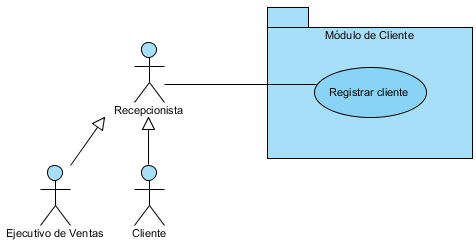
\includegraphics[width=0.8\textwidth]{images/RegistrarCliente}
		\caption{Diagrama de Casos de Uso del sistema.}
	\end{figure}

%\begin{UseCase}[archivo de imágen]{UCX}{Nombre del Caso de uso}{
	\begin{UseCase}{CU1}{Registrar cliente.}{
		Permite registrar los datos de un cliente mayor de 18 años para poder adquirir una membresía. El registro de la información del cliente sólo lo podrá realizar la recepcionista, ejecutivo de ventas y el propio cliente.
	}
		\UCitem{Versión}{0.1}
		\UCitem{Actor}{Ejecutivo de Ventas, Recepcionista y Cliente.}
		\UCitem{Propósito}{Tener un historial sobre las membresías y/o servicios contratados por el cliente.}
		\UCitem{Entradas}{Nombre(s), Apellido Paterno, Apellido Materno, Fecha de Nacimiento, CURP, RFC, Sexo, Calle, Número exterior, Número interior, Colonia, Estado, Delegación/Municipio, Código Postal, Calle anterior, calle Posterior, Referencias, Correo electrónico, Teléfonos, Tipo de sangre, Enfermedades, Condición médica.}
		\UCitem{Origen}{Teclado.}
		\UCitem{Salidas}{Mensaje de registro exitoso, número de cliente, envío de correo electrónico de confirmación a la cuenta de correo del cliente, muestra la \IUref{IU3}{Pantalla de Venta de Membresía}}
		\UCitem{Destino}{Servidor de correo, pantalla.}
		\UCitem{Precondiciones}{No tener registrado otro cliente con la misma CURP y contar con la mayoría de edad (+18).}
		\UCitem{Postcondiciones}{Habrá un cliente más registrado en el sistema.}
		\UCitem{Errores}{{\bf E1:} ``El cliente es menor de edad.'' -- El sistema muestra el Mensaje {\bf MSG1-}``Debes ser mayor de 18 años para continuar con el registro y adquirir tú membresía. Una vez finalizado el registro podrás dar de alta a un afiliado menor de edad'' y continua al paso 1.
		
				{\bf E2:} ``Existe un registro con la misma CURP.'' -- El sistema muestra el Mensaje {\bf MSG2-}``Este cliente ya existe. Ingresa una nueva CURP o consulta los clientes registrados.'' y continua al paso 1.
				
				{\bf E3:} ``No se ingresaron todos los datos obligatorios.'' -- El sistema muestra el Mensaje {\bf MSG3-}``Ingresa los campos obligatorios para continuar'' y continua al paso 3.
				
				{\bf E4:} ``El formato del dato es incorrecto''. -- El sistema muestra el Mensaje {\bf MSG5-}``Ingresa el valor correcto [{\em Formato de dato}]'' y continua en el paso 3.}
		\UCitem{Tipo}{Caso de uso primario}
		\UCitem{Observaciones}{}
		\UCitem{Autor}{Roberto Mendoza Saavedra}
		\UCitem{Revisor}{}
	\end{UseCase}

	\begin{UCtrayectoria}{Principal}
		\UCpaso[\UCactor] Solicita el registro de un cliente seleccionando la opción de ``Registrarse'' de la \IUref{IU2}{Pantalla principal}.
		\UCpaso Solicita los datos del cliente a registrar mostrando la \IUref{IU4}{Pantalla de Registrar Cliente}.
		\UCpaso[\UCactor] Proporciona los datos personales.
		\UCpaso Verifica la mayoría de edad del cliente [E1].
		\UCpaso[\UCactor] Proporciona los datos de la ubicación.
		\UCpaso[\UCactor] Proporciona los datos de contacto.
		\UCpaso[\UCactor] Proporciona los datos médicos.
		\UCpaso[\UCactor] Confirma el registro presionando el botón \IUbutton{Guardar}.
		\UCpaso Verifica que todos los datos marcados como obligatorios en la \IUref{IU4}{Pantalla de Registrar Cliente} se hayan ingresado [E3].
		\UCpaso Verifica que todos los datos proporcionados tengan el formato especificado en el modelo de entidades de acuerdo a su tipo de dato.
		\UCpaso Valida que no exista previamente un registro de cliente con la misma CURP [E1].
		\UCpaso Registra todos los datos proporcionados del cliente.
		\UCpaso Muestra el Mensaje {\bf MSG4-}``Registro exitoso. Tú número de cliente es: [{\em Número de cliente}]''.
		\UCpaso Se dirige a la \IUref{IU3}{Pantalla de Venta de Membresía}.
		
	\end{UCtrayectoria}
	

	
